\section{Walkthrough} \label{sec:walkthrough}
In this section, we introduce \chameleon{} by walking through examples of its
use. The examples are given from the perspective of a hypothetical Haskell 
programmer Maxine. 

\todo{A bit of redundant/repeated here c.f. prev section - if this is Usage example, again use motivating example in it?}

\subsection{Basic mode} \label{sub:basic}
Maxine writes a function to calculate the sum of a list of
numbers, but \chameleon{} shows there is a type error (Fig. \ref{fig:basic-mode-1}). 
After reading error reports, Maxine realized that the error possibly revolves 
around the expression \texttt{xs}.

\begin{figure}[h]
        \centering
        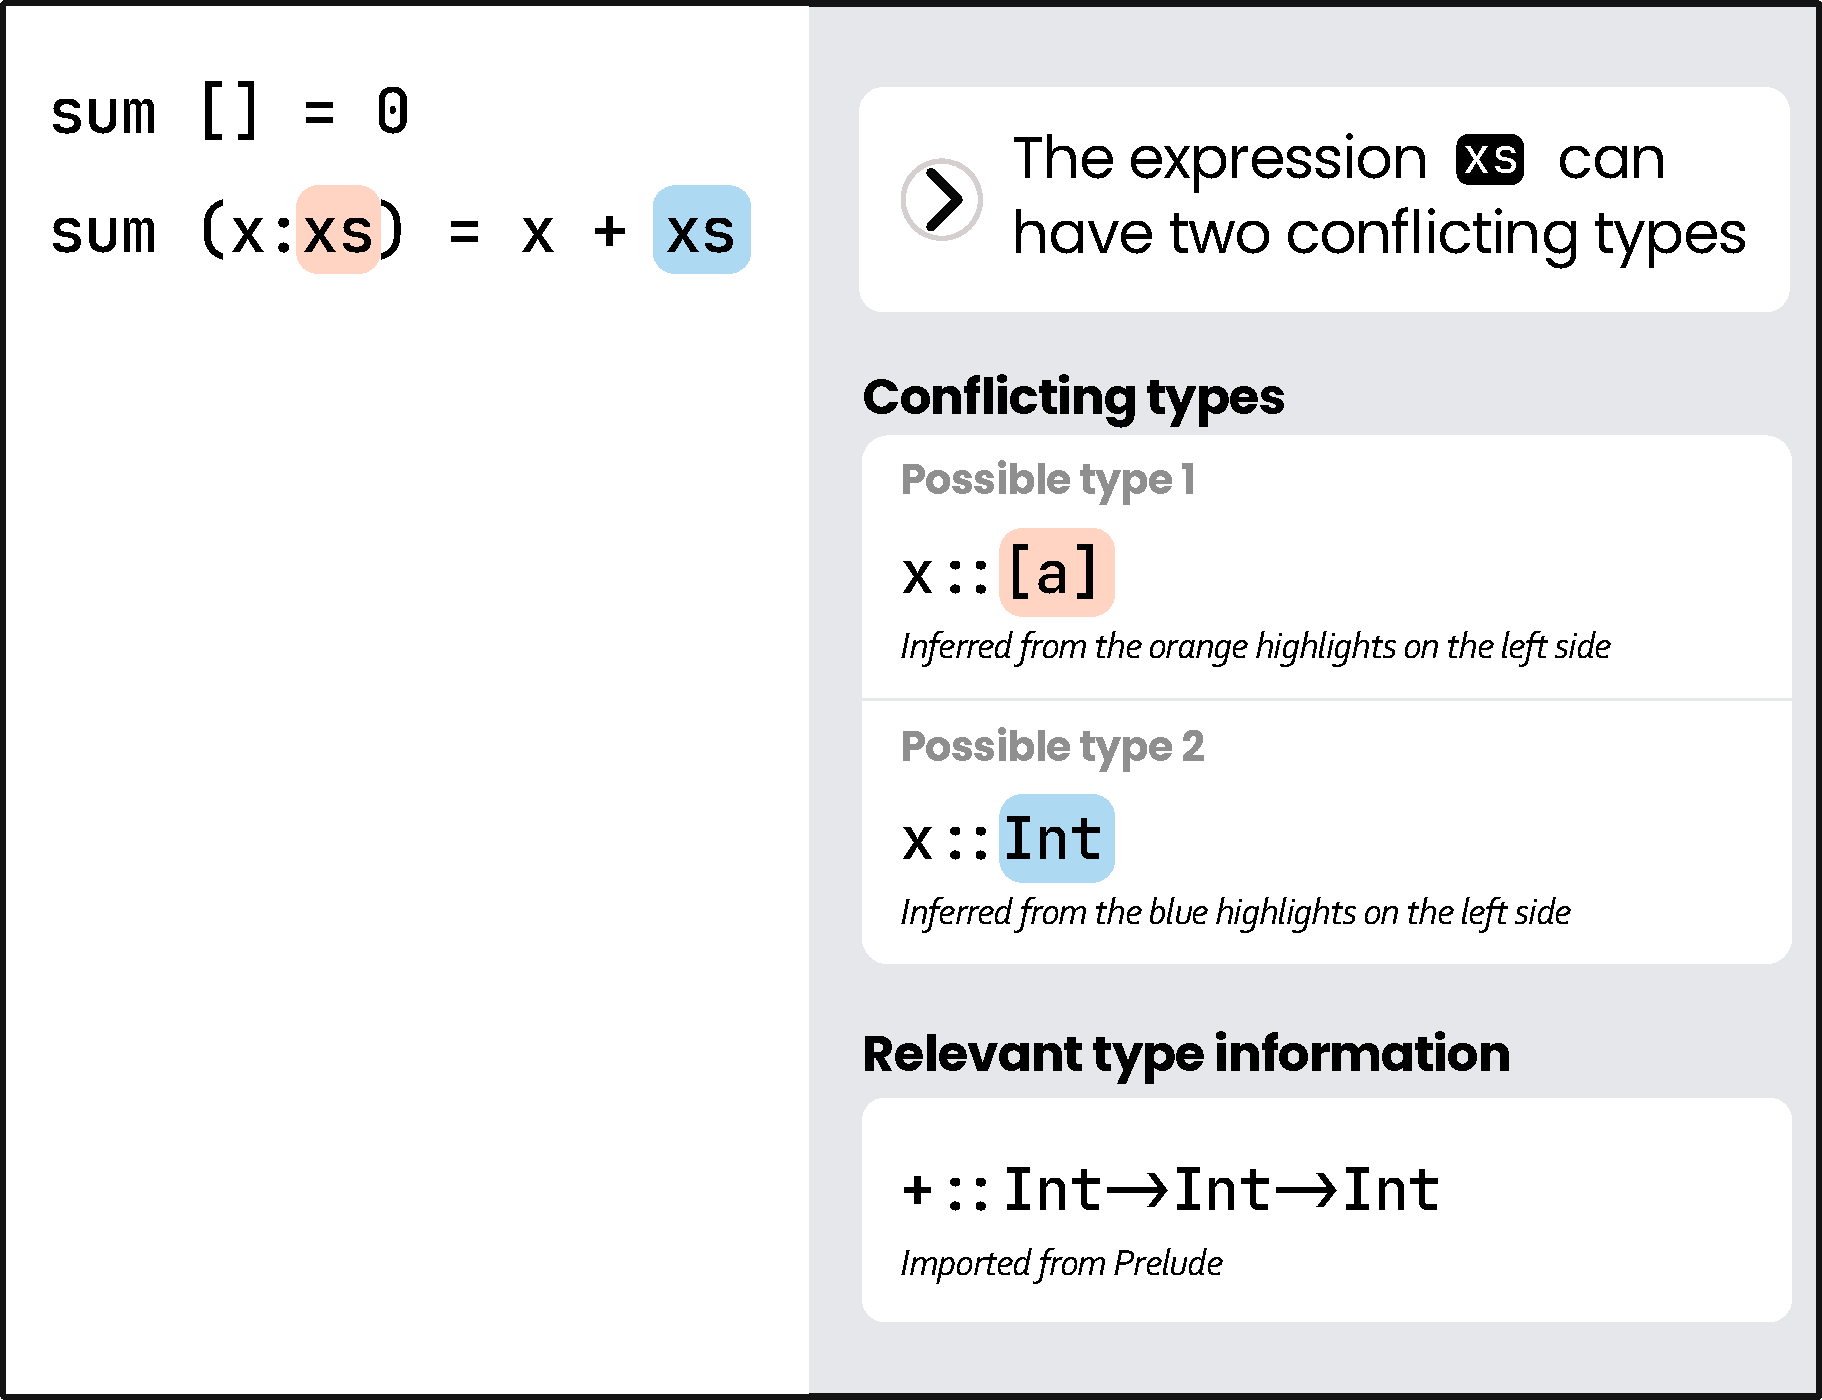
\includegraphics[width=\linewidth]{images/basic-mode-1.pdf}
        \caption{
            Maxine's code to calculate the sum of a list of integers;
            \chameleon{} reports an error on the expression \texttt{xs}.
            }
            \label{fig:basic-mode-1}
\end{figure}

\begin{figure}[h]
        \centering
        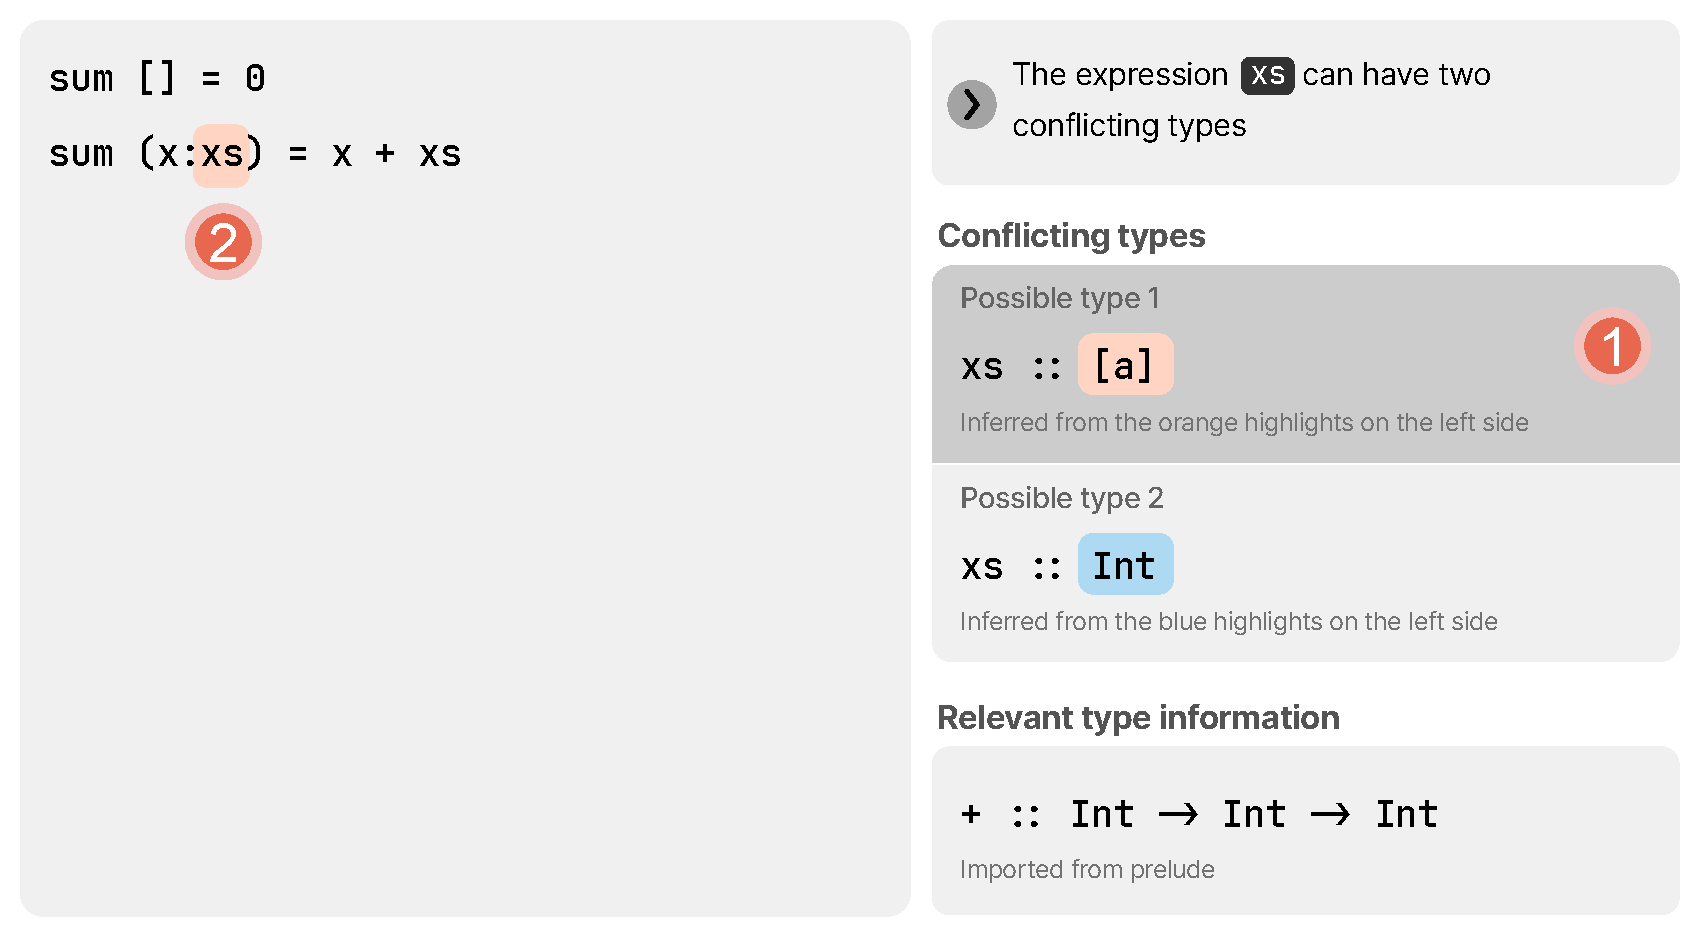
\includegraphics[width=\linewidth]{images/basic-mode-2.pdf}
        \caption{
       Hovering on possible type 1 will limit the highlights 
       in the editor to only the ones (in orange) that support \texttt{x::[a]}.
        }
        \label{fig:basic-mode-2}
\end{figure}

\begin{figure}
        \centering
        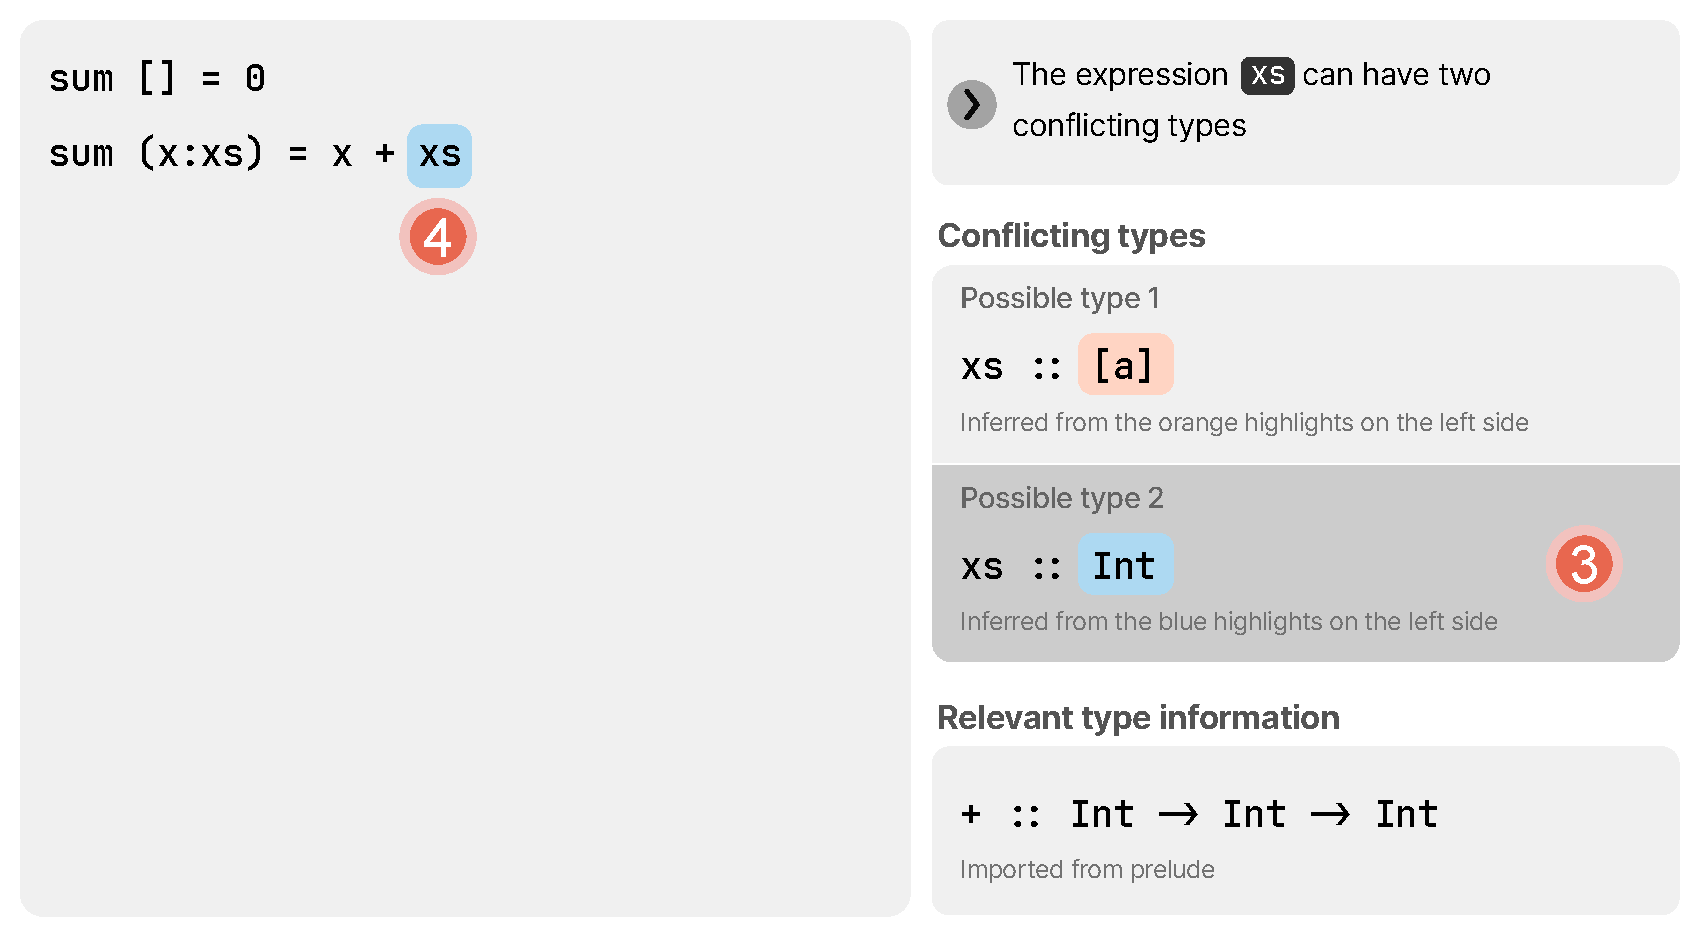
\includegraphics[width=\linewidth]{images/basic-mode-3.pdf}
        \caption{
            Hovering on possible type 2 (Fig. \ref{fig:basic-mode-2}-3) will limit the highlights 
            in the editor to only the ones (in blue) that support \texttt{x::Int}.
        }
        \label{fig:basic-mode-3}
\end{figure}





After scanning the type error report, Maxine realizes that \texttt{xs} can be
either \texttt{[a]} type (Fig. \ref{fig:basic-mode-2}) or \texttt{Int} type (Fig. \ref{fig:basic-mode-2}). By matching the color in the
conflicting type panel (Fig. \ref{fig:anatomy}-G) and the highlighted error locations 
Maxine knows that the \texttt{[a]} type results from the pattern matching of the
\texttt{:} operator, and the \texttt{Int} type results from using \texttt{+} to
 add two expressions. 


At this point, Maxine knows the possible type 1 aligns with her understanding of
the program, and therefore, the error locations with blue highlights must be
erroneous. After examining the program, it is obvious that Maxine missed
applying the \texttt{sum} function recursively at the right-hand side of the
addition. 


\subsection{Balanced mode} \label{sub:balanced}


Maxine writes additional code to add only the even numbers in a list of integers.
In this implementation, Maxine reuses the \texttt{sum} function she wrote
earlier. After saving the file, \chameleon{} shows that there is a type error in the
expression \texttt{sum} (Fig. \ref{fig:balance-mode-1}). However, this is not   \todo{Add annotation to figure like prev ones i.e. (1) so can refer to in text without reader searching for it?}
helpful because Maxine knows that the implementation of  \texttt{sum} is correct 
because it was verified in the previous task. Switching to
balanced mode, Maxine noticed that \chameleon{} shows two cards: \texttt{sum}
and \texttt{evens}. 

\begin{figure}
        \centering
        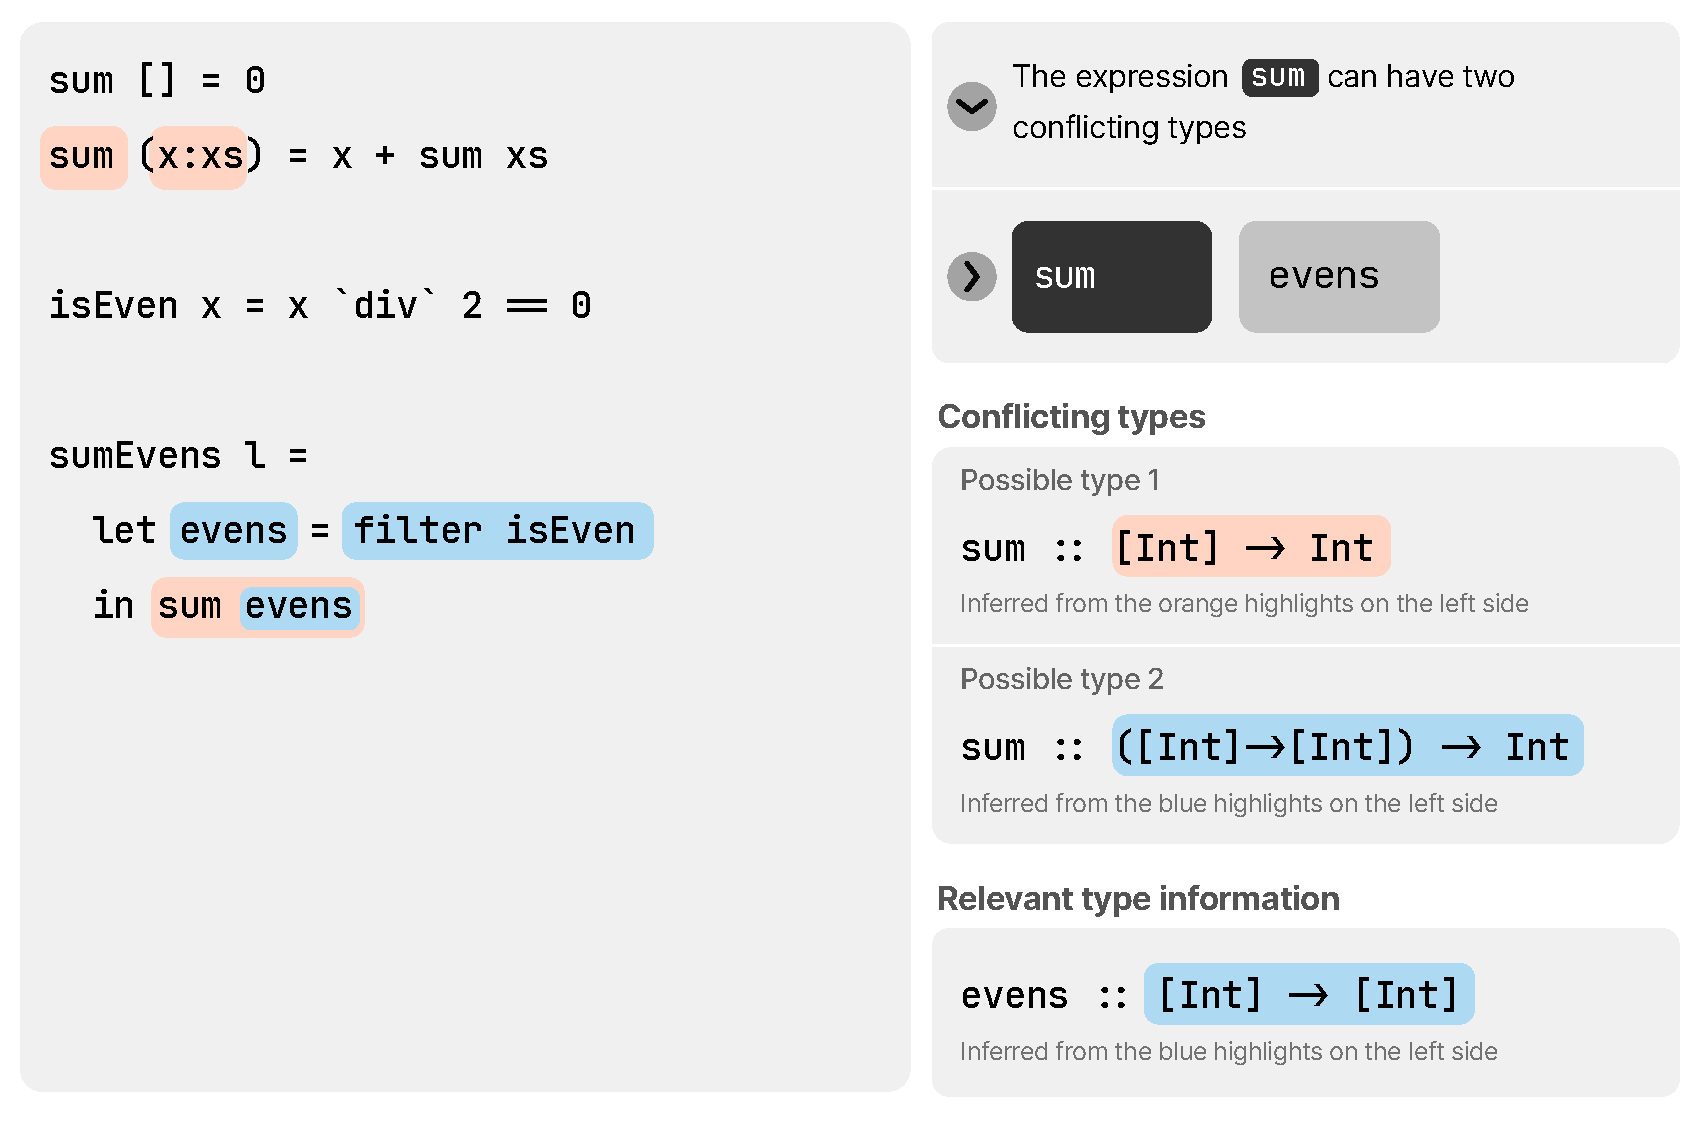
\includegraphics[width=\linewidth]{images/balanced-mode-1.pdf}
        \caption{
            Maxine's code to calculate only the sum 
            of even numbers. \chameleon{} reports 
            an error with two candidate expressions.
        }
        \label{fig:balance-mode-1}
\end{figure}


\begin{figure}
   \centering
        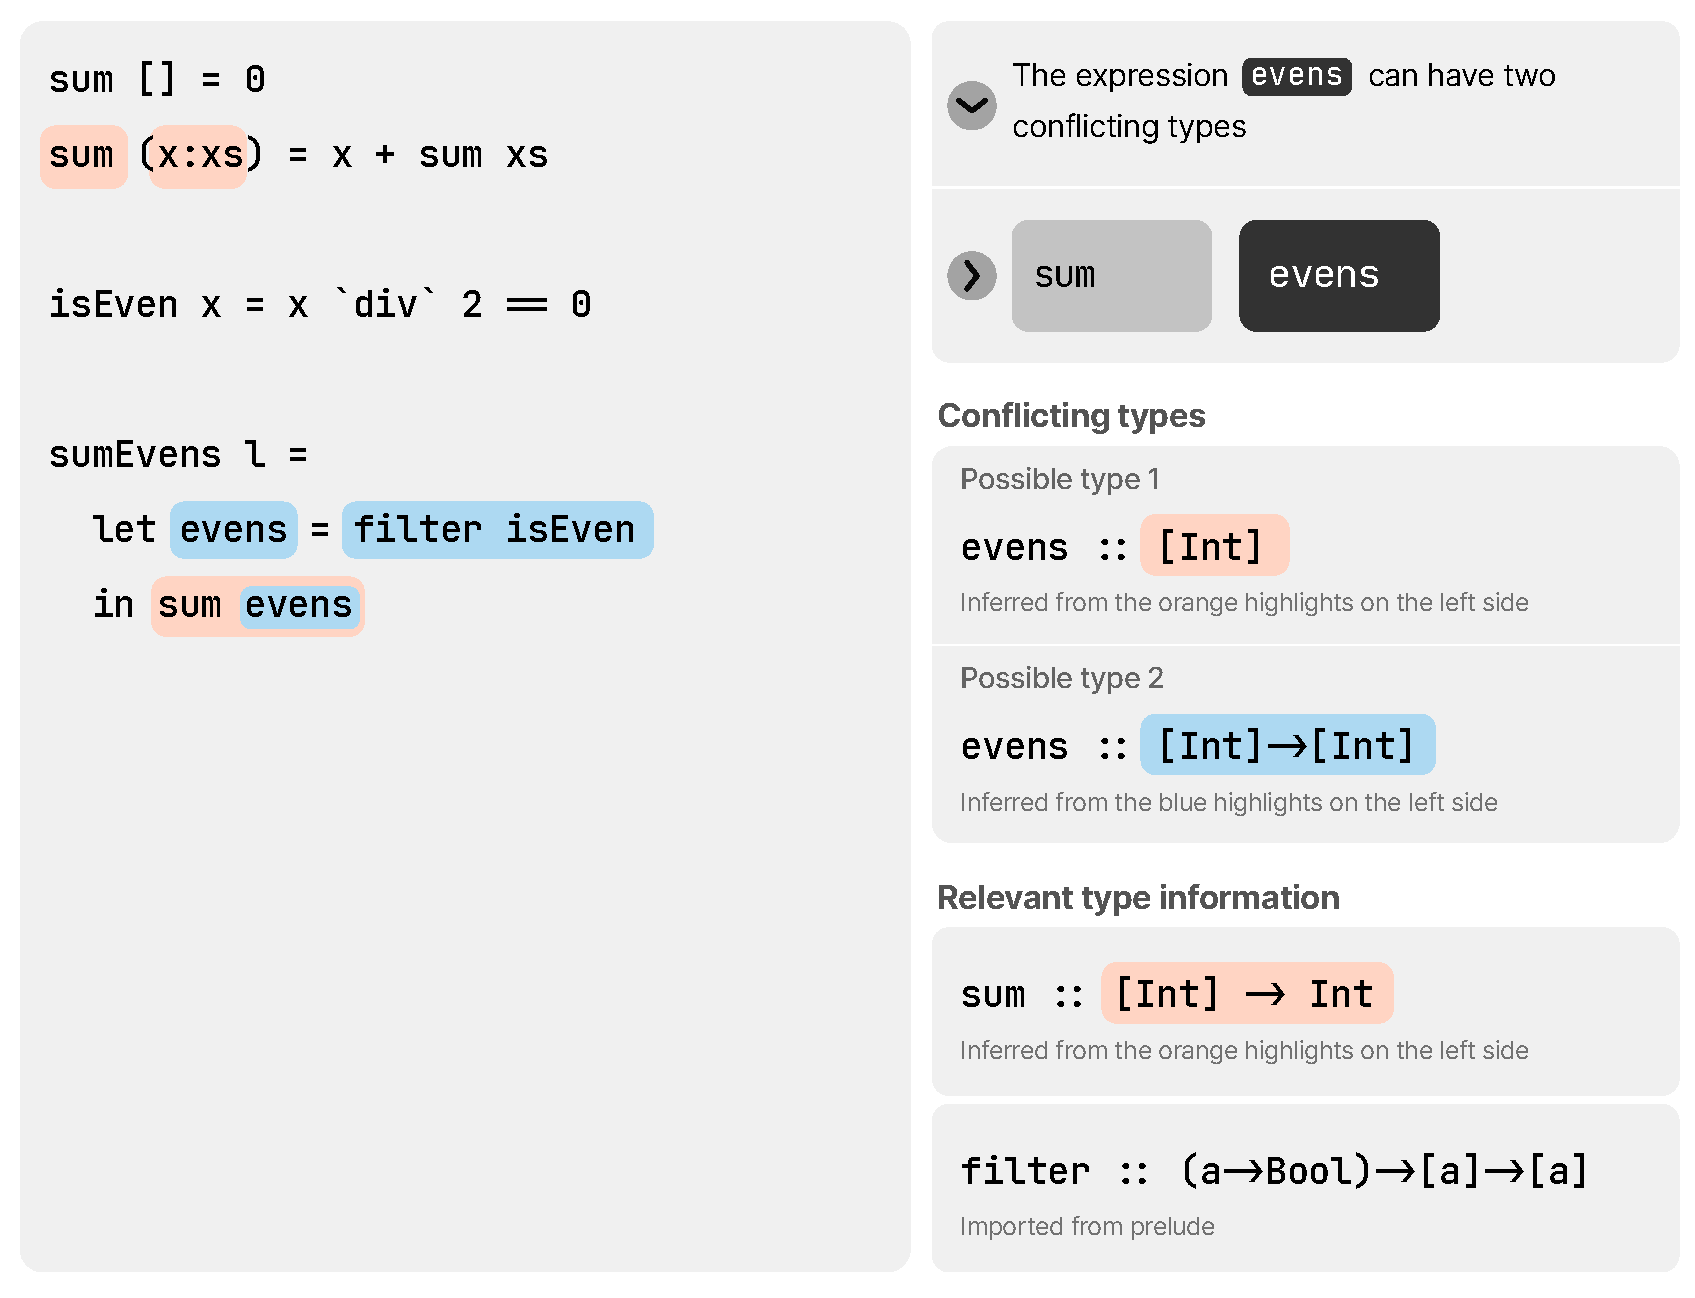
\includegraphics[width=\linewidth]{images/balanced-mode-2.pdf}
        \caption{
            Clicking on the \texttt{evens} card (5) results in the changes in the
            conflicting types panel to show the possible types for \texttt{evens},
            and the changes highlights color to reflect the assumption that the
            definition of \texttt{evens} is the cause of the error.  
        }
        \label{fig:balance-mode-2}
\end{figure}



Maxine therefore clicks on the \texttt{evens} card and \chameleon{} shows two
possible types for the expression \texttt{[Int]} and \texttt{[Int] -> [Int]}
(Fig. \ref{fig:balance-mode-2}). Knowing the expression \texttt{evens} holds
a temporary list of even integers (hence it is of \texttt{[Int]} types), Maxine
knows the Possible type 2 is unintended, and blue in-text highlights must
contain the cause. It does not take long until Maxine realizes that the list 
\texttt{l} is not supplied to the \texttt{filter} function.


\subsection{Advanced mode}  \label{sub:advanced}


For the task shown in section \ref{sub:balanced}, if Maxine is not satisfied by
the options provided by \chameleon{}, by switching to advanced
mode, Maxine has access to the debugging steps and the explanation layer. 

\begin{figure}
        \centering
        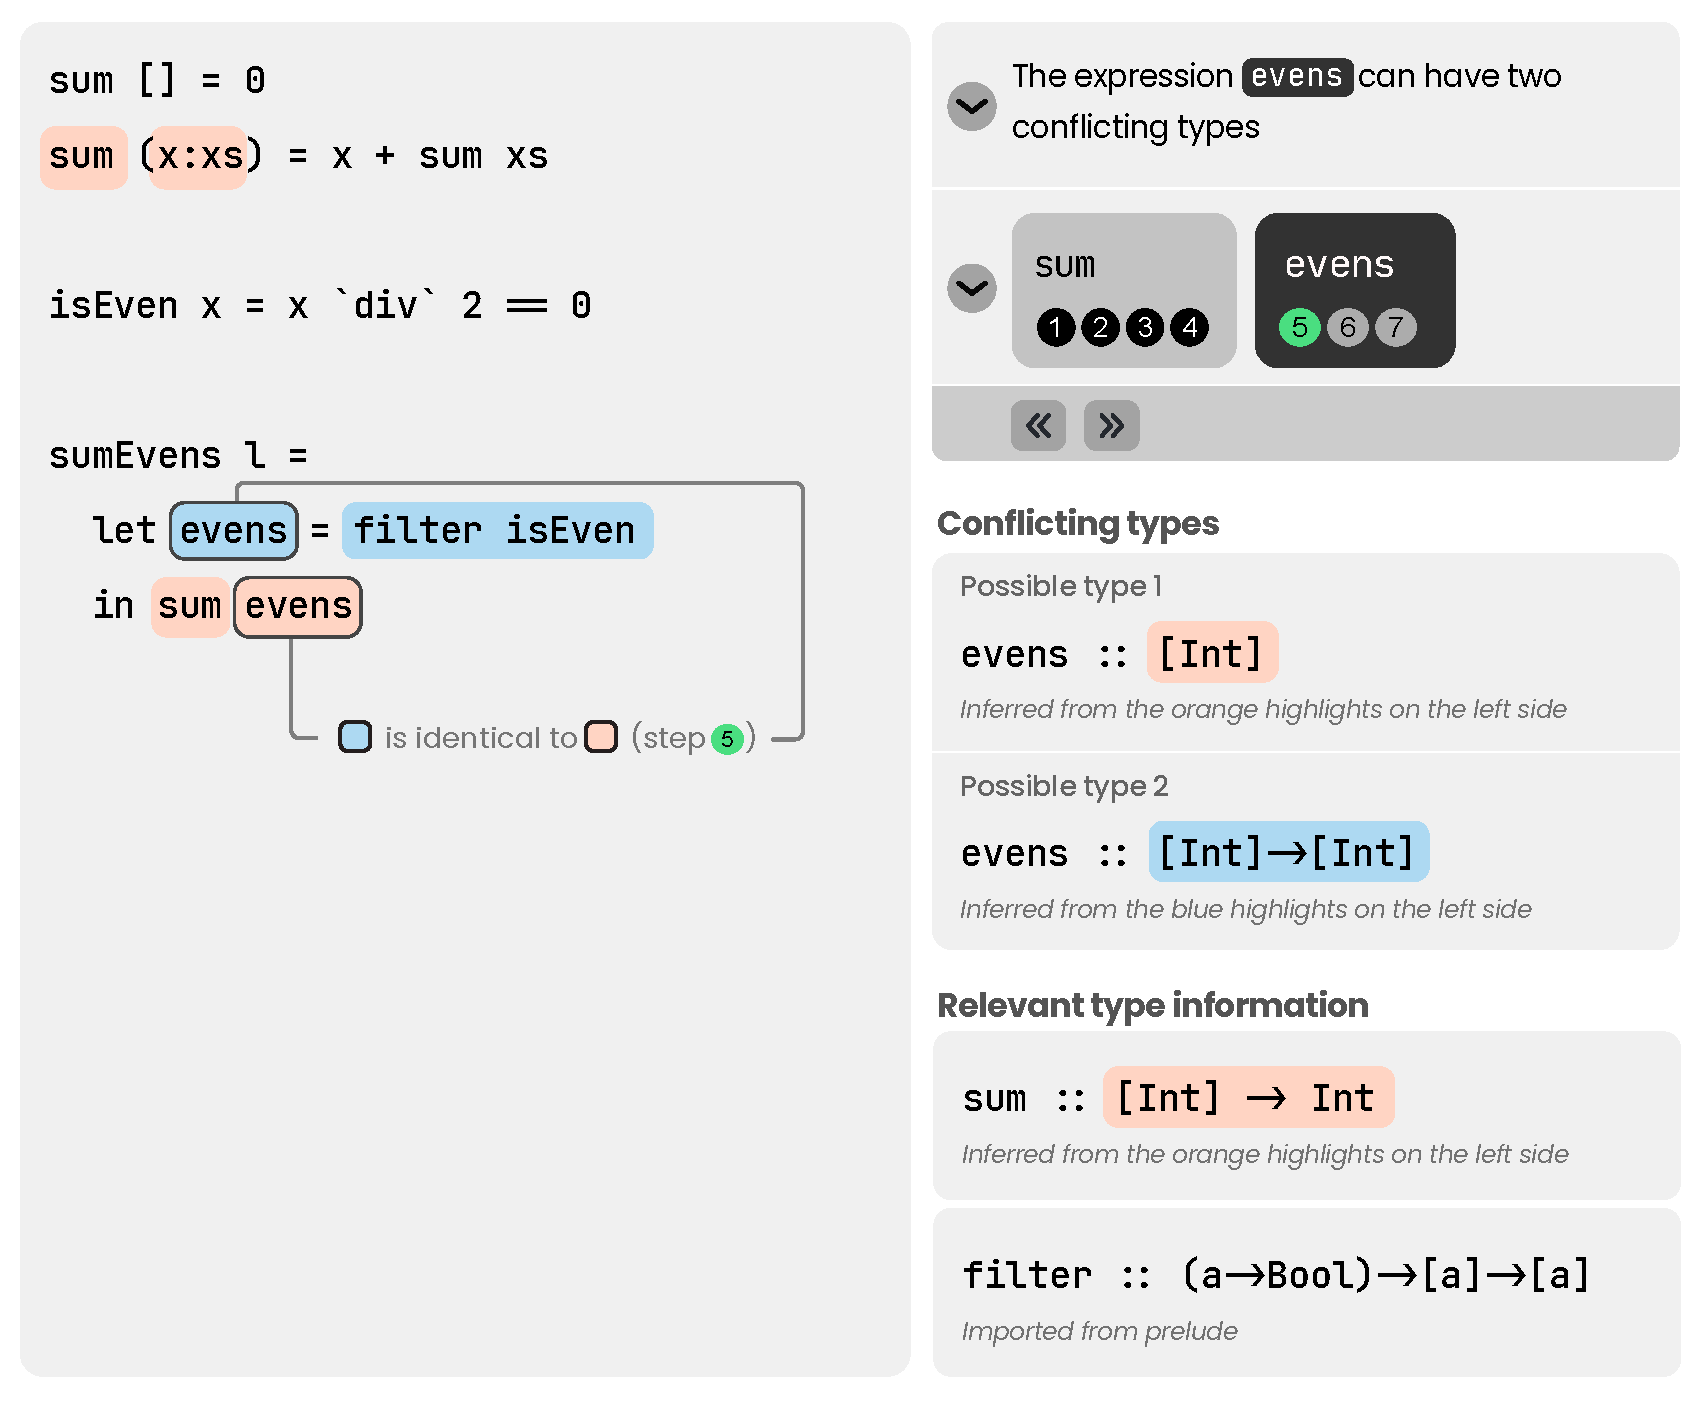
\includegraphics[width=\linewidth]{images/advanced-mode-1.pdf}
        \caption{
            Maxine's code to calculate only the sum 
            of even numbers in advanced mode. 
            The current step is step 5, \chameleon{} 
            explains that the two appearances of expression 
            \texttt{evens} should have the same type.
        }
        \label{fig:advanced-mode-step5}
\end{figure}

\begin{figure}
        \centering
        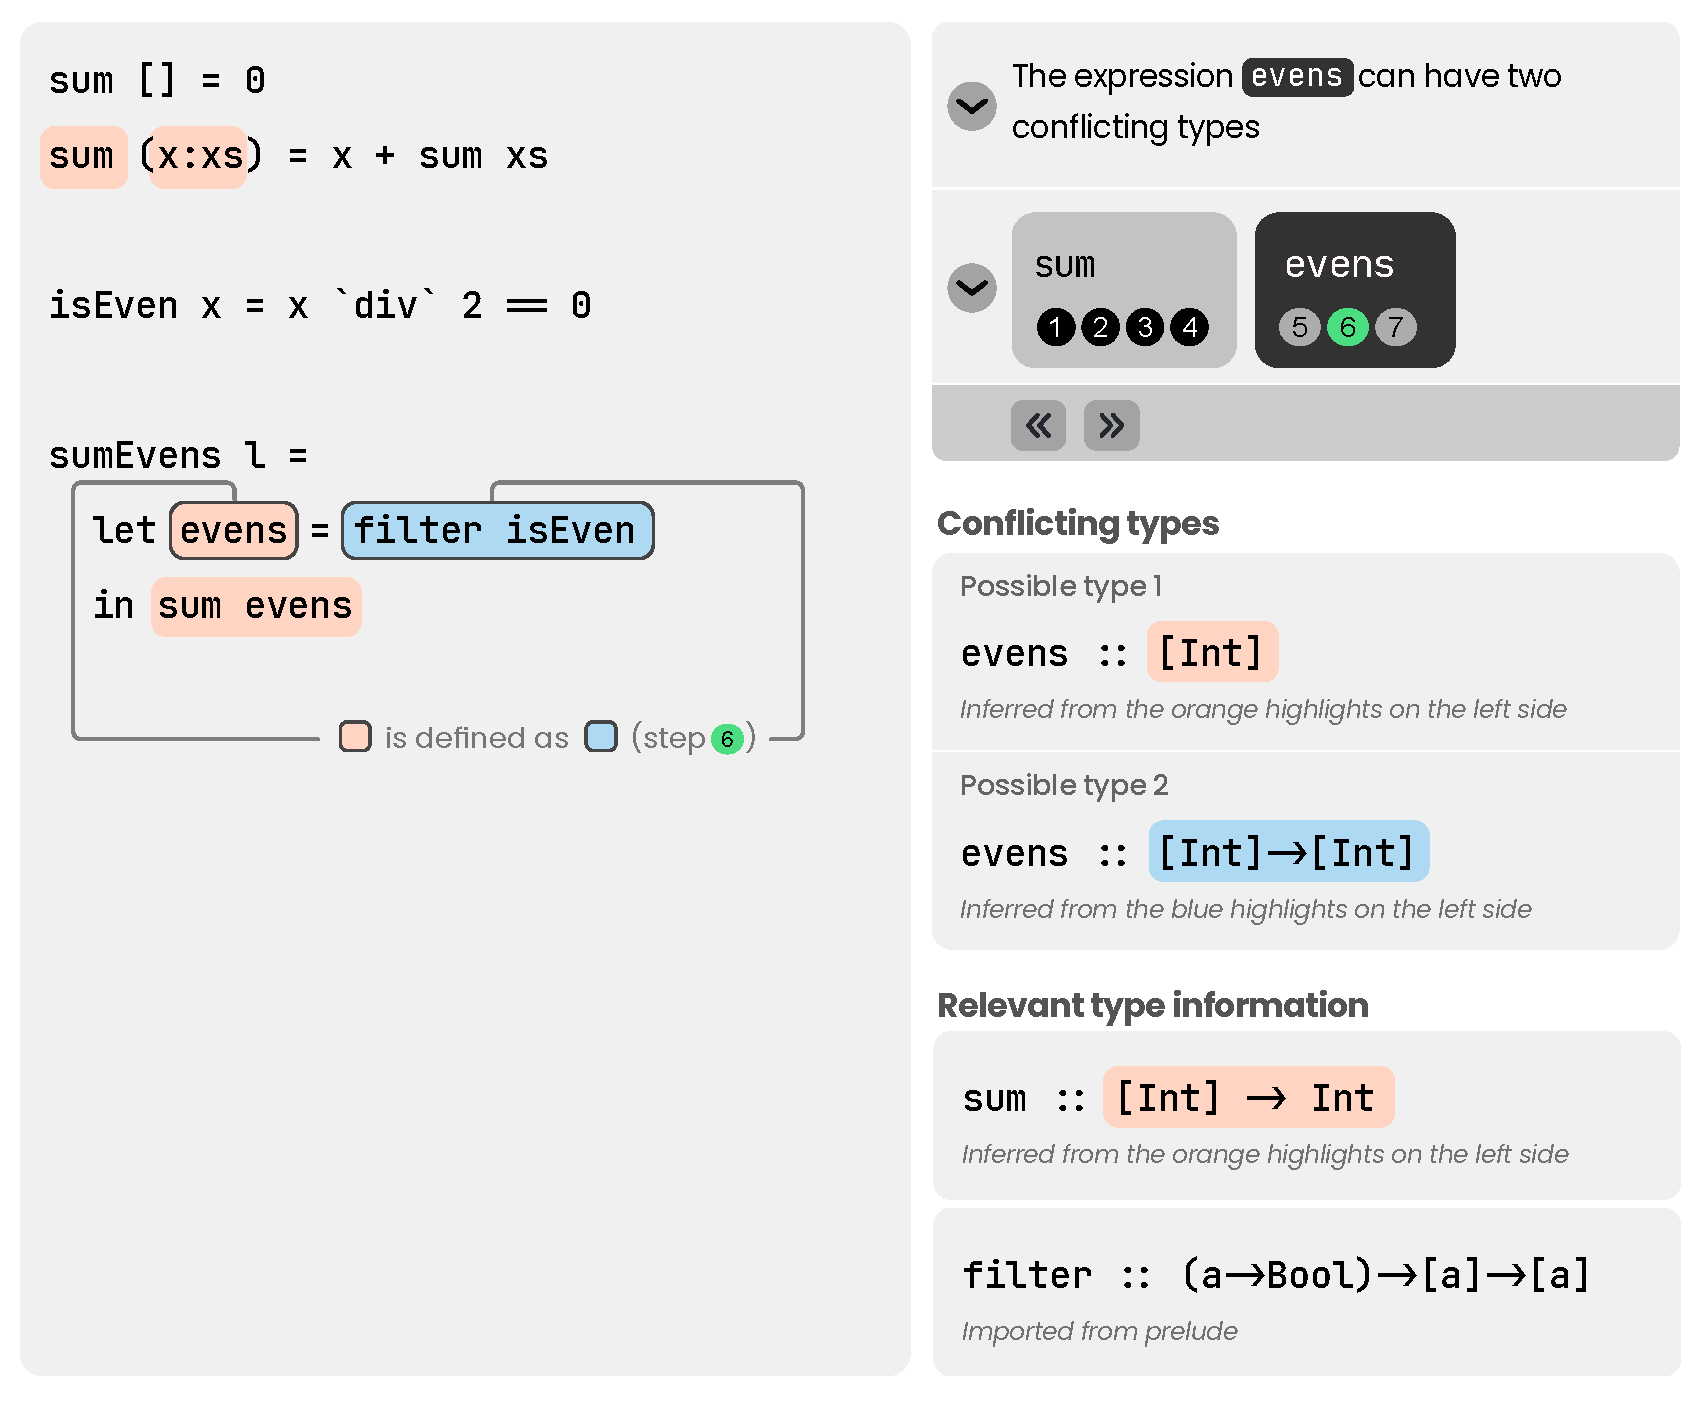
\includegraphics[width=\linewidth]{images/advanced-mode-2.pdf}
        \caption{
            In step 6, \chameleon{} 
            explains that \texttt{evens} is defined as
            the expression \texttt{filter isEven}. The left-hand side
            and right-hand side should have the same type.
        }
        \label{fig:advanced-mode-step6}
\end{figure}

\begin{figure}
        \centering
        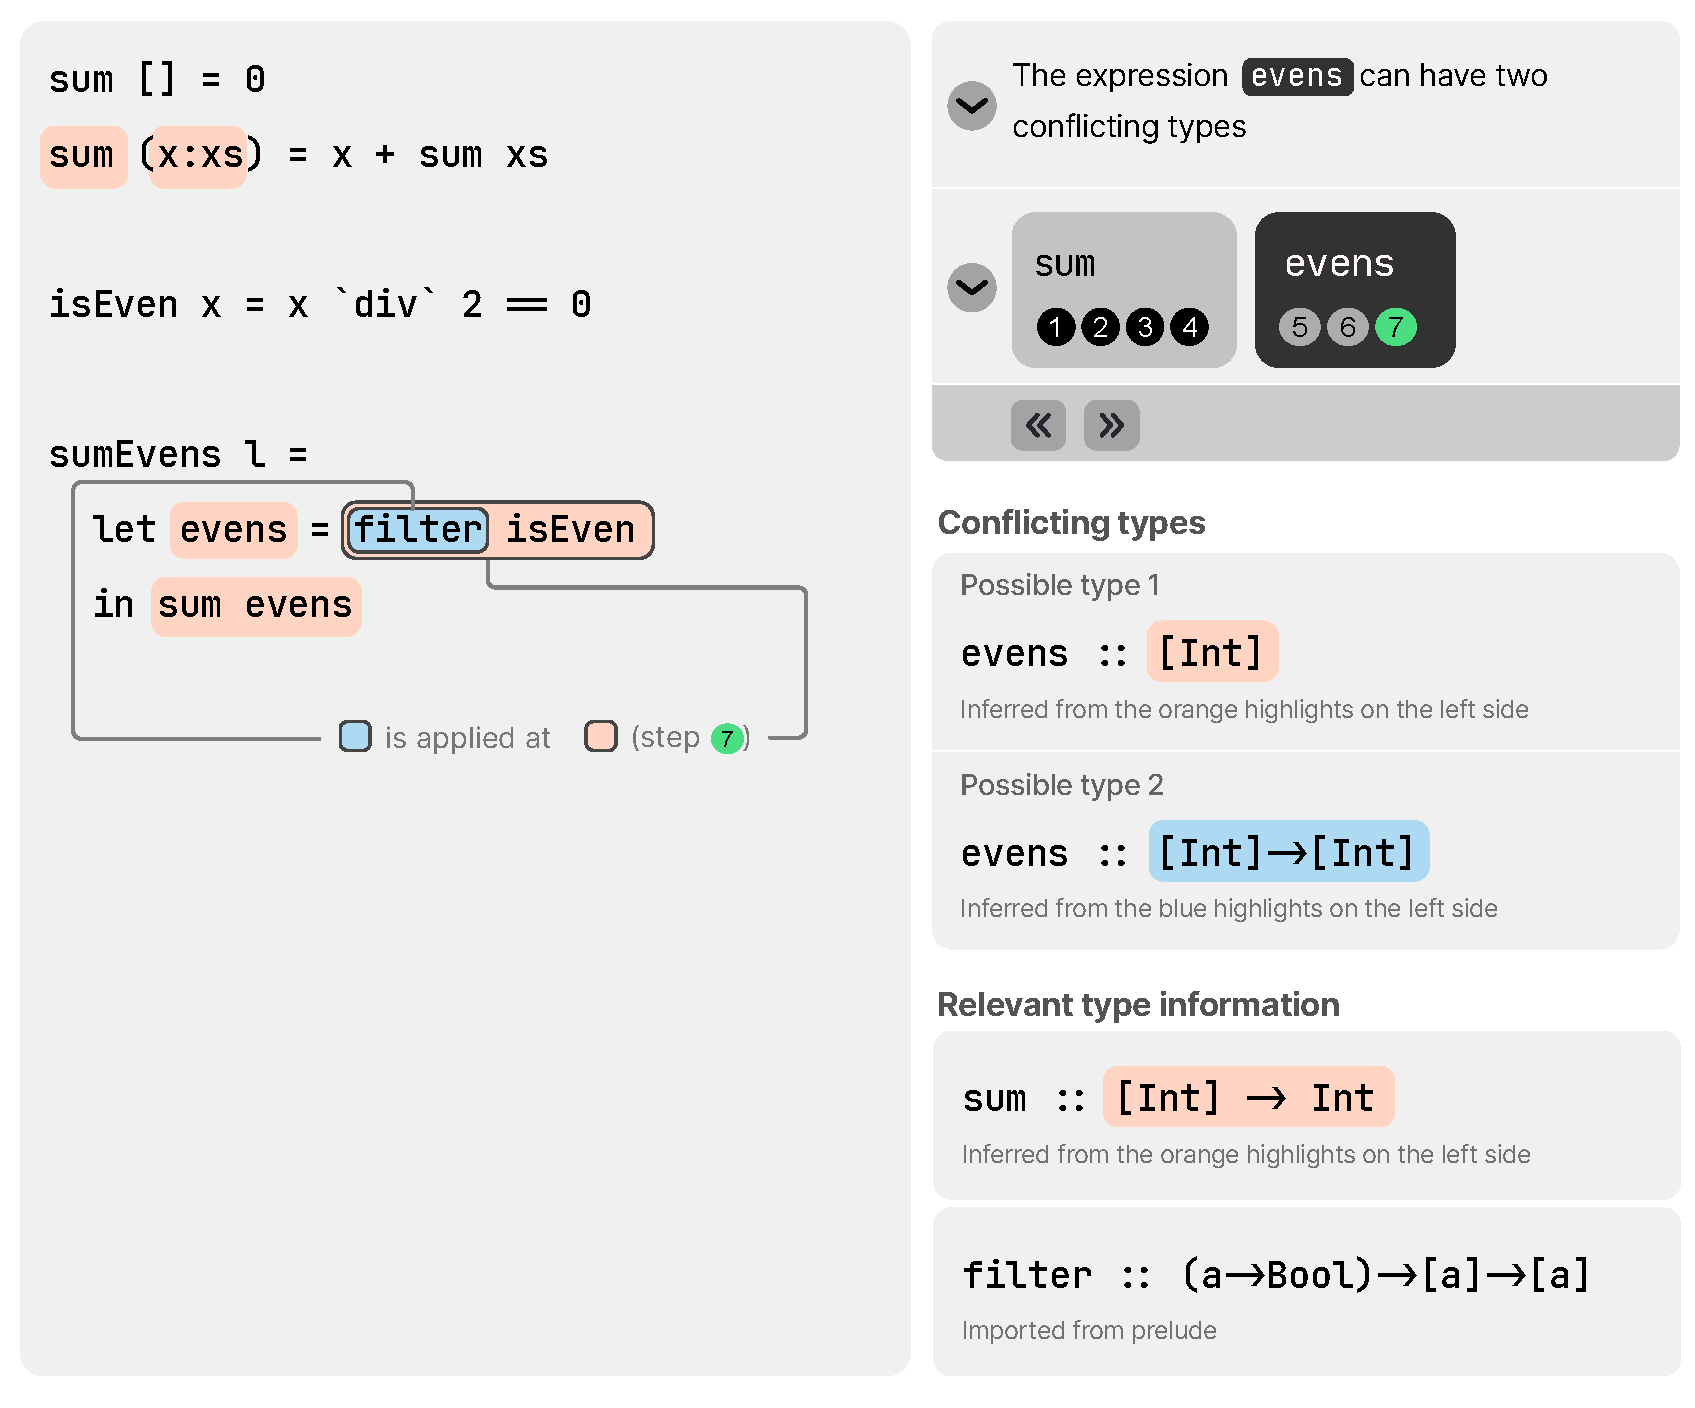
\includegraphics[width=\linewidth]{images/advanced-mode-3.pdf}
        \caption{
            In step 7, \chameleon{} 
            explains that \texttt{filter} is applied to 
            the function \texttt{isEven}. Assisting by 
            the type of \texttt{filter} in the 
            Relevant Type Information panel on the bottom
            right, Maxine can find the type error that 
            \texttt{filter} expects two arguments but receives one.
        }
        \label{fig:advanced-mode-step7}
\end{figure}



First, Maxine clicks on step 5 (Fig. \ref{fig:advanced-mode-step5}) and verifies
that the two occurrences of \texttt{evens} are supposed to be identical, and the
second usage dictates that \texttt{evens} is a list of integers. Second, she
clicks on step 6 (Fig. \ref{fig:advanced-mode-step6}) and verifies that
\texttt{evens} should be the same type as the declaration on the right-hand
side. 


Lastly, Maxine clicks on step 7 (Fig. \ref{fig:advanced-mode-step7}), and
it shows that the \texttt{filter} function is applied to one argument
\texttt{isEven}. By consulting the relevant type information, Maxine identifies
that \texttt{filter} is expecting two arguments while only one is provided. 

